\chapter{Introduction}
\label{intro}
Particle physics seeks to understand the fundamental constituents of nature and their interactions. At the present moment, the Standard Model of particle physics (along with the general theory of relativity) represents the most complete understanding humanity has yet achieved. At the same time, the Standard Model cannot explain gravity or several observed but not yet understood aspects of nature and therefore must give way to a more complete theory at a higher energy scale. One approach to understanding what might be hiding beneath the Standard Model is to use high-energy particle collisions to probe nature at ever smaller length scales. This thesis presents a search for beyond the Standard Model physics in \SI{13}{\TeV} proton-proton collision data collected by the Compact Muon Solenoid experiment at the Large Hadron Collider, which is the highest-energy particle collider ever constructed.

The search presented in this thesis targets new long-lived particles that produce displaced leptons, a unique signature that could evade many existing searches for new physics. In this chapter, I present theoretical context in the form of a brief overview of the Standard Model and targeted discussion of beyond the Standard Model physics and long-lived particles. I then present the experimental context with an overview of the Large Hadron Collider and the Compact Muon Solenoid detector in Chapter~\ref{lhc_and_cms}, present the search itself in Chapter~\ref{displaced_leptons}, and conclude in Chapter~\ref{conclusion}. 

\section{The Standard Model}
The Standard Model of particle physics (SM) describes all known particles and their non-gravitational interactions. Developed and experimentally verified over the past six decades, the SM posits the existence of twelve spin-$\frac{1}{2}$ particles, the fermions, that make up all observed matter; twelve spin-1 particles, the gauge bosons, that communicate the electromagnetic, weak, and strong forces; and one fundamental scalar, the Higgs boson, which breaks electroweak symmetry, giving mass to the gauge bosons and fermions.

The fermions and gauge bosons can be classified according to the forces with which they interact. The fermions are further divided into six quarks, which carry color and interact via the strong force, and six leptons, which do not. Furthermore, all six quarks and three of the leptons carry electric charge and interact electromagnetically (the neutral leptons are called neutrinos). All fermions interact via the weak force. The gauge bosons include the photon, which communicates the electromagnetic force; the $\mathrm{W}^+$, $\mathrm{W}^-$, and $\mathrm{Z^0}$, which communicate the weak force; and eight gluons that communicate the strong force. Of these, only the $\mathrm{W}^+$ and $\mathrm{W}^-$ are electrically charged and only the gluons carry color charge. Finally, the fermions are grouped into three generations, each with two quarks, one charged leptons, and one neutral lepton. Figure~\ref{sm_particles} diagrams the grouping of the SM particles and lists some of their properties.
\fxnote{cite something}

\begin{figure}
\centering
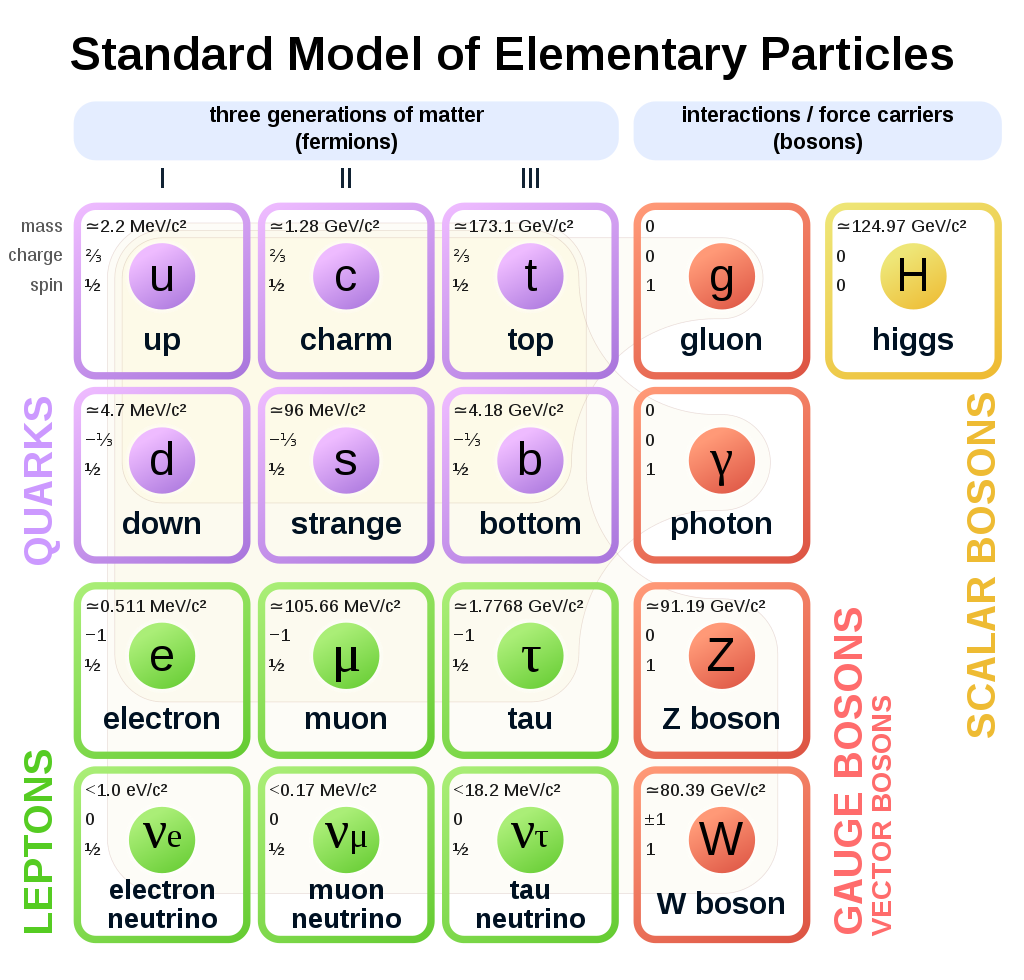
\includegraphics[scale=0.4]{figures/intro/sm_particles.png}
\caption{The Standard Model particle content.}
\label{sm_particles}
\end{figure}

In the SM, the interactions between particles are governed by two theories: quantum chromodynamics (QCD), which describes the strong force, and the electroweak theory, which describes the electromagnetic and weak forces. The following sections will provide a brief overview of these theories.

\subsection{Quantum chromodynamics}
QCD describes the strong interactions between quarks and gluons and is based on the $SU(3)_{c}$ symmetry group, where the subscript c refers to color charge. In QCD, all quarks and gluons carry color charge, which allows interactions between two quarks of the same generation and a gluon, three gluons, or four gluons. QCD is responsible for the formation of all hadrons (such as protons and neutrons), and leads to two unique phenomena: confinement and asymptotic freedom. \fxnote{quarks transform as triplets, 3 color charges, developed in the 70s, ?}

Confinement refers to the experimental fact that an isolated particle with color charge has never been directly observed. Composite particles composed of quarks and gluons are always neutral under color, and attempts to separate the constituent particles will only produce new hadrons. This phenomenon is the result of the unique running of the strong coupling constant, which increases with decreasing energy (and therefore increasing distance). \fxnote{energy, momentum transfer, interaction energy?} \fxnote{mention dis?} \fxnote{mention jets?}

Asymptotic freedom shows up at the opposite end of the energy spectrum. In high energy interactions (such as those at the Large Hadron Collider), the strong coupling constant is small enough to render the quarks nearly free. In this regime, the small coupling constant enables perturbative calculations. \fxnote{say why this matters, especially if it matters for lhc stuff}

\subsection{The electroweak theory}
The electroweak theory unifies the electromagnetic and weak interactions and is based on the $SU(2)_{L} \otimes U(1)_{Y}$ symmetry group. It posits two new charges: weak isospin, which has three components $T_{1,2,3}$, and hypercharge, $Y$. $T_{3}$ is $\pm\frac{1}{2}$ for all left-handed fermions and 0 otherwise, while Y varies according to $Q=T_{3}+\frac{1}{2}Y$, where $Q$ is the familiar electric charge. Each generation of left-handed quarks or leptons forms an SU(2) doublet. The first generation doublets, for example, are:
\begin{equation}
    \binom{\nu_{e}}{e^{-}}_{L},\ \binom{u}{d}_{L}
\end{equation}
where, as in $SU(2)_{L}$, the L denotes left-handed chiral states. The three generators of $SU(2)_{L}$ result in three massless spin-1 bosons: $W1$, $W2$, and $W3$, while $U(1)_{Y}$ gives rise to one massless spin-1 boson, $B^{0}$. When all is said and done, the physical $W^{\pm}$ bosons are identified as superpositions of $W^{1}$ and $W^{2}$ while $Z^0$ and the photon are identified as superpositions of $W^{3}$ and $B^{0}$.

Terms in the electroweak Lagrangian\fxnote{shit, do I have to introduce Lagrangians somewhere?} involve either two left-handed fermions and a $W^{\pm}$ or $Z^{0}$, two electrically charged particles and a photon, or charge-conserving combinations of $W^{\pm}$s, $Z^{0}$s, and photons that include three or four particles. \fxnote{does it make sense to talk about this in terms of physical states before introducing ssb?} Conspicuously missing, however, are mass terms for the electroweak gauge bosons or fermions.
\fxnote{cp violation, mixing between generations, right-handed neutrinos?}
\fxnote{needs citations}

\subsection{The Higgs mechanism}
As shown in Fig.~\ref{sm_particles}, the fermions and $W^{\pm}$ and $Z^{0}$ bosons all have nonzero mass. Accounting for this fact within the context of QCD and the electroweak theory is difficult because explicit mass terms violate the gauge and chiral\fxnote{define chiral?} symmetry of $SU(3)_{c} \otimes SU(2)_{L} \otimes U(1)_{Y}$. For example, a term such as
\begin{equation}
    \frac{1}{2}m_{A}^{2}A^{\mu}A_{\mu},
\end{equation}
which assigns mass $m_{A}$ to gauge boson $A$, becomes
\begin{equation}
    \frac{1}{2}m^{2}(A^{\mu}-\partial^{\mu}\alpha)(A_{\mu}-\partial_{\mu}\alpha) \neq \frac{1}{2}m^{2}A^{\mu}A_{\mu}
\end{equation}
under a $U(1)$ gauge transformation\fxnote{double check language, define alpha}, and a term such as
\begin{equation}
    m_{f}\overline{f}f = m_{f}(\overline{f}_{R}f_{L} + \overline{f}_{L}f_{R}),
\end{equation}
which assigns mass $m_{f}$ to fermion $f$, breaks chiral symmetry by coupling the right- and left-handed components of the fermion.\fxnote{is coupling them really the problem, or is it that they are being treated identically?}

If the gauge and chiral symmetries of $SU(3)_{c} \otimes SU(2)_{L} \otimes U(1)_{Y}$ truly are symmetries of nature and the fermions and $W^{\pm}$ and $Z^{0}$ bosons truly have nonzero mass, then another mechanism must be at work. Spontaneous symmetry breaking, which occurs when the vacuum state\fxnote{of what?} does not exhibit\fxnote{have?} all of the symmetries of the underlying theory. In such a situation, each spontaneously broken continuous symmetry gives rise to a massless scalar particle \cite{goldstone_salam_weinberg}. In the case of spontaneously broken continuous \textit{gauge} symmetries, however, there exists a mechanism by which the massless bosons are removed and some of the gauge bosons associated with the generators of the symmetries acquire mass \cite{englert, higgs, kibble}. In the SM, this mechanism, known as the Higgs mechanism, breaks electroweak symmetry, gives mass to the fermions and $W^{\pm}$ and $Z^{0}$ bosons, and results in one massive scalar particle, the Higgs boson.

The Higgs mechanism adds the scalar doublet
\begin{equation}
    \Phi = \binom{\phi^{+}}{\phi^{0}},
\end{equation}
whose potential is given by
\begin{equation}
    V(\Phi^{\dagger}\Phi) = \mu^{2}\Phi^{\dagger}\Phi + \lambda(\Phi^{\dagger}\Phi)^{2},
\end{equation}
to the SM. If $\mu^{2}<0$ and $\lambda>0$, then $\Phi^{\dagger}\Phi = -\frac{\mu^{2}}{2\lambda}$ defines a circle of minima in the $\phi^{+}$--$\phi^{0}$ plane. Even though the potential remains invariant under $SU(2)_{L} \otimes U(1)_{Y}$, nature must spontaneously choose a vacuum state somewhere along this circle. Because the vacuum state does not respect $SU(2)_{L} \otimes U(1)_{Y}$, the symmetry is said to be spontaneously broken.

This procedure has three significant consequences. First, three of the four\fxnote{why are only three generators broken?} degrees of freedom originally associated with $\Phi$ are now associated with the longitudinal components of the $W^{\pm}$ and $Z^{0}$ bosons, which causes them to acquire mass while the photon remains massless. Second, $\Phi$'s remaining degree of freedom adds a single massive scalar, the Higgs boson, to the theory. Third, the interaction between the fermions and the nonzero vacuum state of the scalar field produces fermion mass terms that obey chiral symmetry.
\fxnote{describe how we're left with U(1)_{em}?}
\fxnote{is it ok to keep glossing over neutrinos?}
\fxnote{do I really understand why fermion yukawa terms obey chiral symmetry?}


\subsection{Current status}
\label{sm_status}
The SM is remarkable successful. It describes all known particles and their non-gravitational interactions, and experiments over the last several decades have repeatedly verified every major prediction it makes.\fxnote{would be nice to walk through experimental history} In 2012, the CMS and ATLAS experiments verified its last major untested prediction by independently discovering an approximately \SI{125}{\GeV} scalar particle with properties consistent with the SM Higgs boson \cite{cms_higgs, atlas_higgs}. Further measurements in \num{7}, \num{8}, and \SI{8}{\TeV} proton-proton collisions at the Large Hadron Collider continue to agree with SM predictions of the Higgs boson properties \fxnote{cite some recent higgs summary}. We finally have meaningful evidence as to the origin of electroweak symmetry breaking, and all current evidence indicates that SM Higgs mechanism is indeed responsible.

Despite this remarkable success, the SM is not without problems. For one, it cannot be the whole story: it says nothing on the subjects of gravity, dark matter, or dark energy, which implies that it only describes about 5\% of the energy content of the universe \fxnote{cite something} and that a more complete theory must take over at or below the energy scale where gravity becomes important ($M_{P}\approx\SI{e16}{\GeV}$) \fxnote{check and cite something}. Furthermore, many aspects of the SM seem arbitrary and unmotivated. It offers no explanation, for example, for why three generations of fermions are necessary or why its many parameters take the values they do. It could be that these unmotivated values are simply experimental facts of nature without explanation, but the history of science implies that a deeper understanding is likely hiding beneath the surface. Finally, the observed value of the Higgs boson mass is not only unexplained, it is unnatural. This final issue, which is explained in the following paragraphs, is a powerful motivation to search for new physics at currently accessible energy scales.

\subsubsection{Naturalness}
The naturalness criterion states that an effective theory such as the SM must not be overly sensitive to the details of the underlying higher energy theory. Put another way, it requires that any dimensionless parameter much smaller than one must be protected by a custodial symmetry \fxnote{cite giudice and/or 't hooft}. Such a criterion may or may not be respected by nature, but history and simple probability are on its side.

The dimensionless parameter in question is the mass of the Higgs boson, which is quadratically sensitive to $\Lambda$, the energy scale at which a new theory takes over. All SM parameters\fxnote{really all?} are affected by interactions with virtual particles through loop diagrams such as those shown in Fig.~\ref{loop_diagrams}, but the Higgs mass is particularly sensitive. As a fundamental scalar, the Higgs boson lacks the chiral and gauge symmetries enjoyed by the fermions and gauge bosons. These symmetries, known as custodial symmetries, protect the fermion and gauge boson masses by guaranteeing that all corrections are proportional to the bare masses themselves\fxnote{I never defined 'bare mass'}. If the SM is indeed valid up $M_{P}$, then the bare mass of the Higgs boson must be coincidentally equal and opposite to the sum of the terms that correct it to approximately one part in \num{e30}. Such miraculous fine tuning is technically possible, but it could also be strong evidence that a deeper physical mechanism is at work.

\begin{figure}[hbtp]
\centering
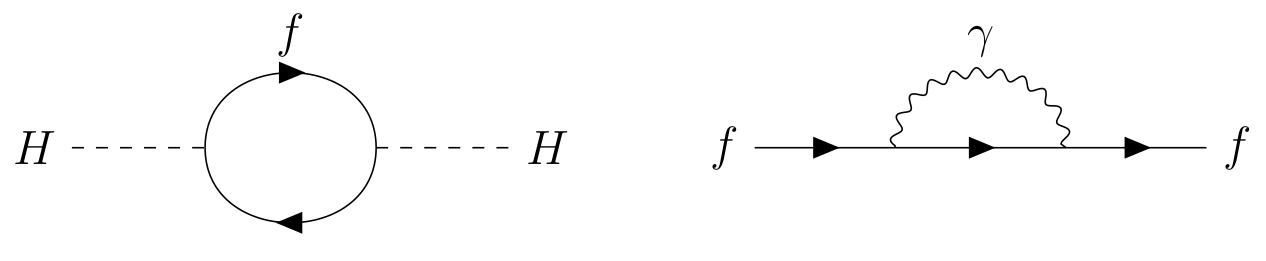
\includegraphics[scale=0.3]{figures/intro/loop_diagrams.png}
\caption{The Higgs boson mass corrected by a fermion loop (left) and a fermion mass corrected by photon loop (right).}
\label{loop_diagrams}
\end{figure}

\fxnote{make sure I don't refer to the Higgs mass when I really mean the square of the Higgs mass}

\section{Beyond the Standard Model}
Many beyond the SM (BSM) theories have been proposed to address the issues discussed in Section~\ref{sm_status}. Theories such as large extra dimensions address the unnatural Higgs boson mass by allowing gravity to spread across more than three spatial dimensions, which lowers $M_P$ and therefore the size of the Higgs boson mass corrections \cite{add}. Other theories posit new symmetries that protect the Higgs boson mass from large corrections. The following section explains supersymmetry, which protects the Higgs boson mass with a new symmetry between bosons and fermions.

\subsection{Supersymmetry}
\label{susy}
Supersymmetry (SUSY) introduces a new symmetry in which every SM particle fits into a larger multiplet with an inherent symmetry between bosons and fermions. In its simplest form, SUSY predicts one new boson for every SM fermion, one new fermion for every SM boson, and one new Higgs doublet. The increase in particle multiplicity necessitates a new naming convention: the spin-0 superpartners of the SM fermions are called sfermions (e.g. sleptons or squarks) while the spin-$\frac{1}{2}$ superpartners to the SM bosons add "ino" to the end of their SM counterpart (e.g. Higgsino or wino).

When calculating contributions to the Higgs boson mass from loop diagrams, one finds that fermion loops differ in sign from boson loops, which means that in SUSY every bosonic correction to the Higgs boson mass is cancelled by a fermionic correction and vice versa. If SUSY were an exact symmetry of nature, the cancellation would be perfect, and the observed Higgs boson mass would match the bare Higgs boson mass exactly \cite{susy_primer}. Figure~\ref{higgs_top_stop_corrections} shows a sample leading-order cancellation.

\begin{figure}[hbtp]
\centering
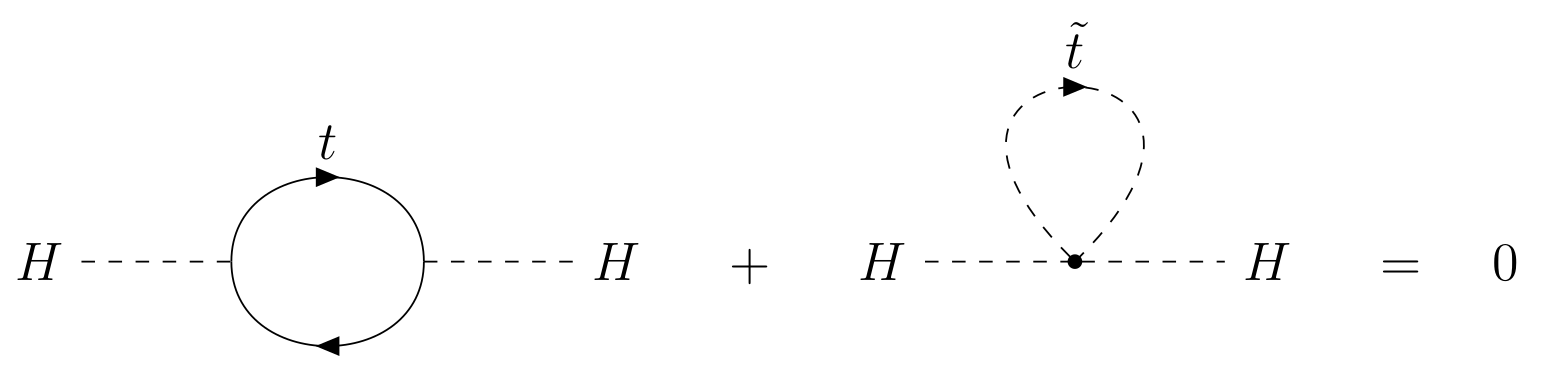
\includegraphics[scale=0.2]{figures/intro/higgs_top_stop_corrections.png}
\caption{Corrections to the Higgs boson mass from the top quark (left) and top squark (right) cancel in exact SUSY. The top quark and top squark contributions are enhanced by the large top--Higgs coupling.}
\label{higgs_top_stop_corrections}
\end{figure}

Exact SUSY also requires that SUSY particles have the same mass as their SM counterparts, so the uniformly null results in collider searches imply that if SUSY exists, it must be a broken symmetry. In broken SUSY, the diagrams in Fig.~\ref{higgs_top_stop_corrections} no longer exactly cancel. Instead, the resulting correction is proportional to the mass of the top squark \cite{craig_susy_run1}, which means that broken SUSY can still resolve the naturalness problem if the masses of the SUSY particles that correct the Higgs boson mass are themselves approximately at the weak scale (say $\mathcal{O}(\SI{250}{\GeV}$)). Many natural SUSY scenarios are therefore excluded as collider experiments set increasingly large lower bounds on SUSY particle masses. Figure~\ref{cms_susy_summary}, for example, shows that the exclusion bounds on top squark and gluino masses extend above \SI{1}{\TeV} in several recent CMS analyses. 

\begin{figure}
\centering
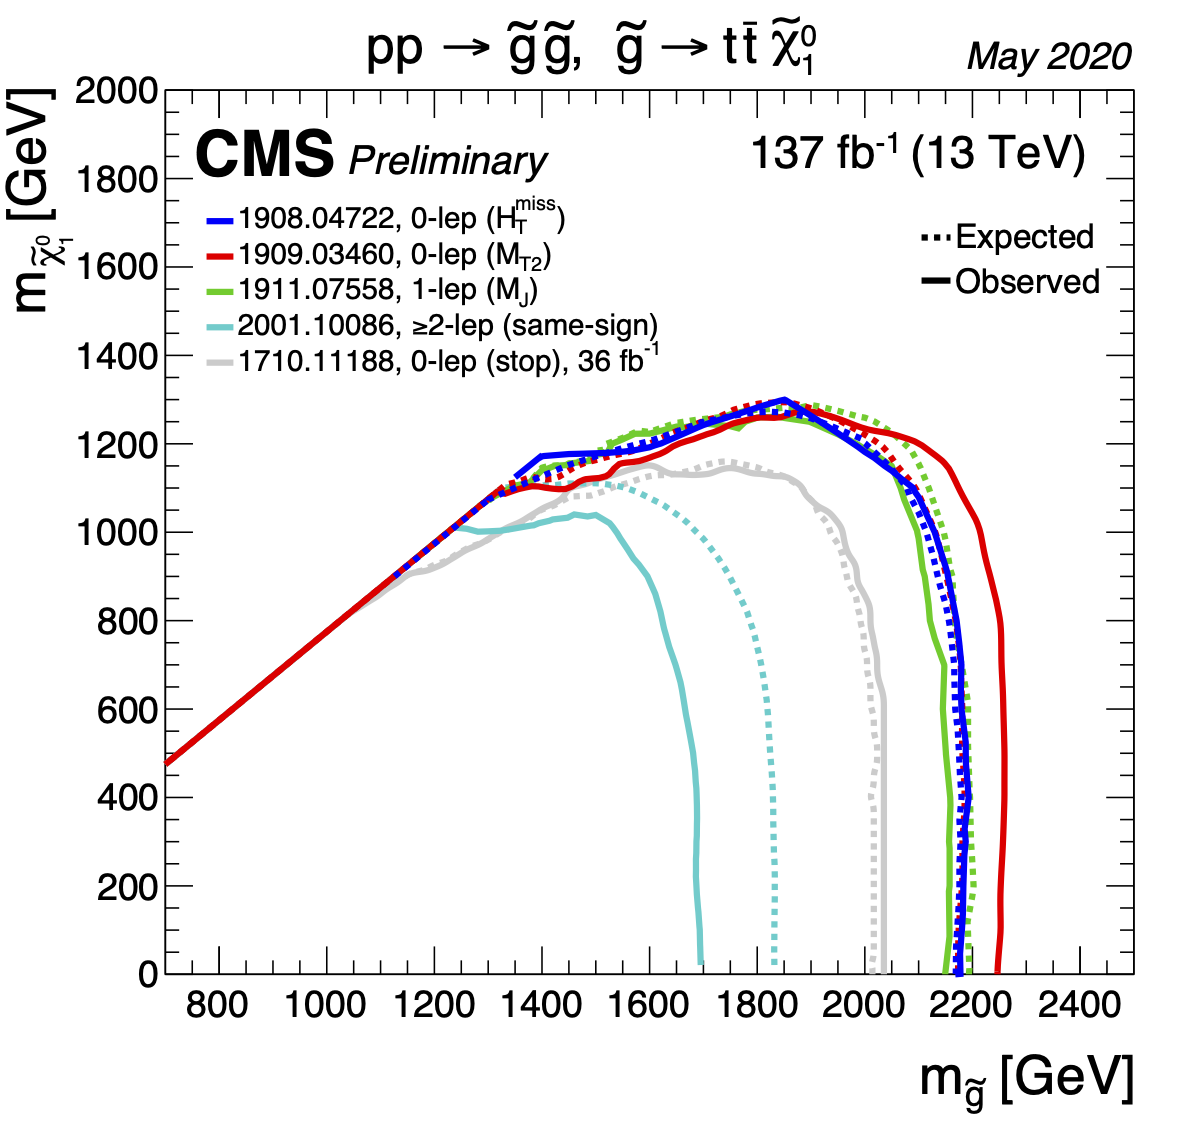
\includegraphics[width=0.45\textwidth]{figures/intro/gluino_mass_limits.png}
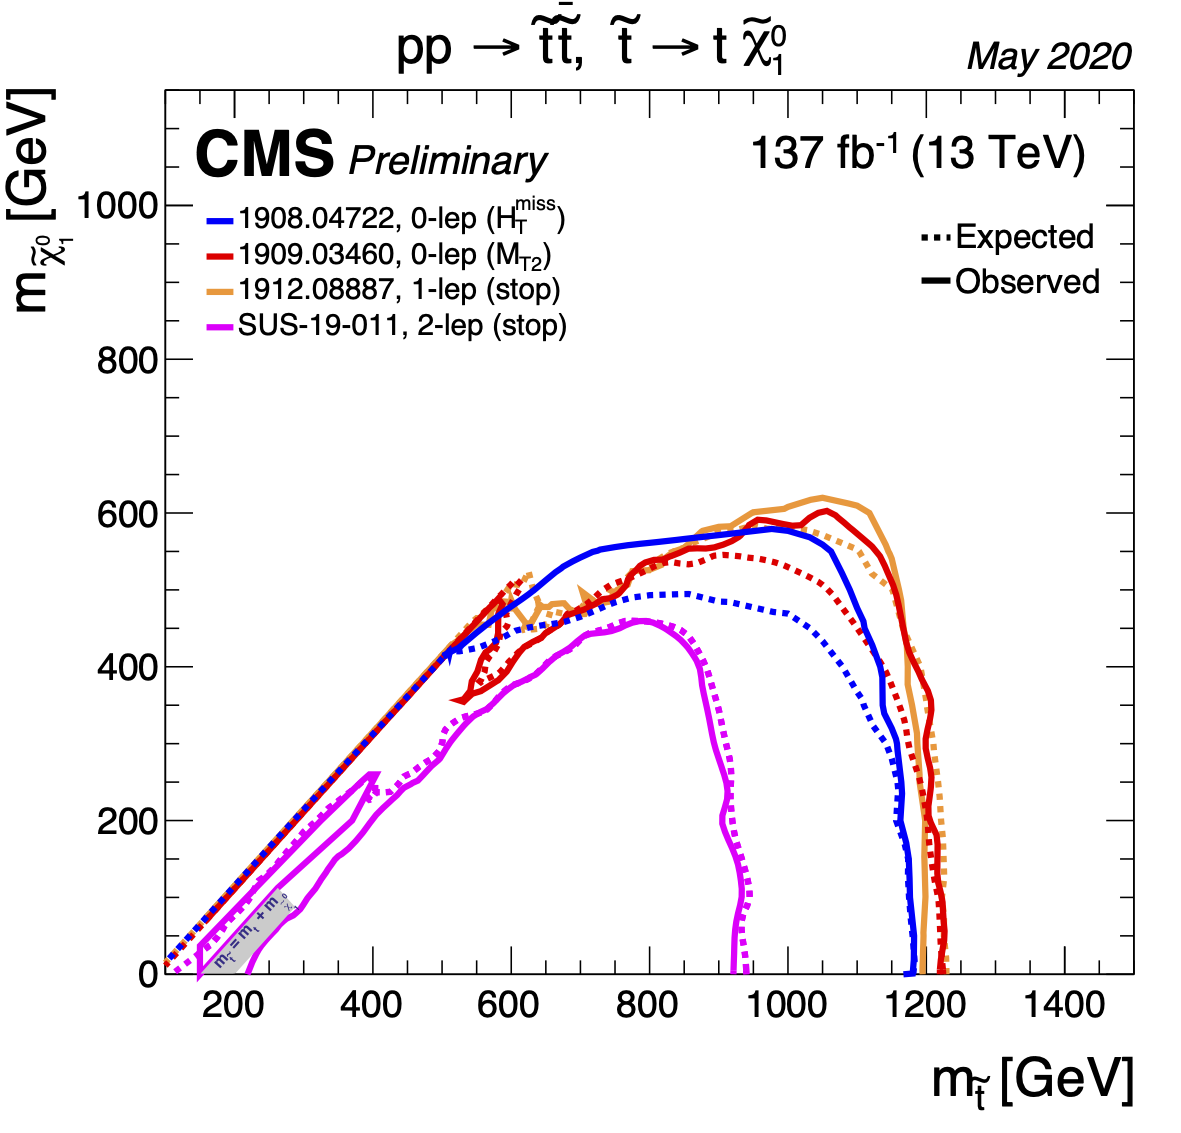
\includegraphics[width=0.45\textwidth]{figures/intro/stop_mass_limits.png}
\caption{Mass limits at \SI{95}{\percent} CL for a simplified model of gluino pair production with gluino decays to pairs of top quarks and the LSP (left) and top squark pair production with squark decays to a top quark and the LSP (right) from several CMS analyses~\cite{cms_susy_public_results}.}
\label{cms_susy_summary}
\end{figure}

As the available natural SUSY parameter space is further constricted, it is important to investigate signatures of new physics that conventional analyses may be missing. One possibility, new long-lived particles, is presented in the following section.

\fxnote{mention gauge coupling, dark matter candidate, etc?}

\subsection{Long-lived particles}
\label{llps}
In the context of collider physics, long-lived particles (LLPs) are particles whose lifetimes are such that they decay a measurable distance from the collision point. This category includes everything from particles that decay less than \SI{1}{\mm} away from the collision to particles that propagate through the entire detector. As shown in Fig~\ref{sm_llps}, long-lived particles are common in the SM.

\begin{figure}[hbtp]
\centering
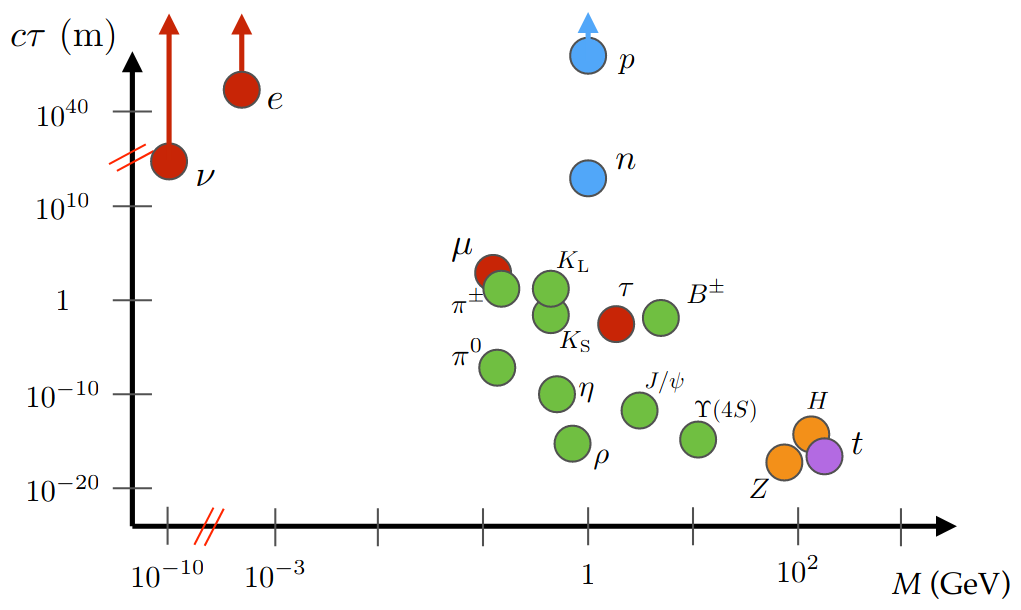
\includegraphics[scale=0.4]{figures/intro/sm_llps.png}
\caption{Masses and proper decay lengths of many Standard Model particles. Particles with proper decay lengths above approximately \SI{e-4}{\m} will be noticeably long-lived in collider detectors such as CMS.\fxnote{cite https://indico.cern.ch/event/607314/contributions/2542308/attachments/1447888/2231430/LHC-LLP_Shuve.pdf}}
\label{sm_llps}
\end{figure}

Long-lived SM particles arise from several mechanisms. First, symmetries such as charge and baryon number conservation ensure that particles such as electrons and protons are absolutely stable. Second, small coupling constants and highly virtual intermediate states decrease the decay rate of particles such as muons, whose \SI{2.2}{\us} lifetime is the product of a weak decay through a virtual $W$ boson (the $W$ boson mass is about \num{760} times that of the muon). Finally, limited decay phase space increases the lifetime of particles such as the neutron, whose decay into a proton, an electron, and an electron neutrino is slowed by the near mass degeneracy of the neutron and the proton. The mass difference between the neutron and its decay products is less than \SI{1}{\MeV}. The muon and neutron decays are diagrammed in Fig.~\ref{neutron_muon_decays}.

\begin{figure}
\centering
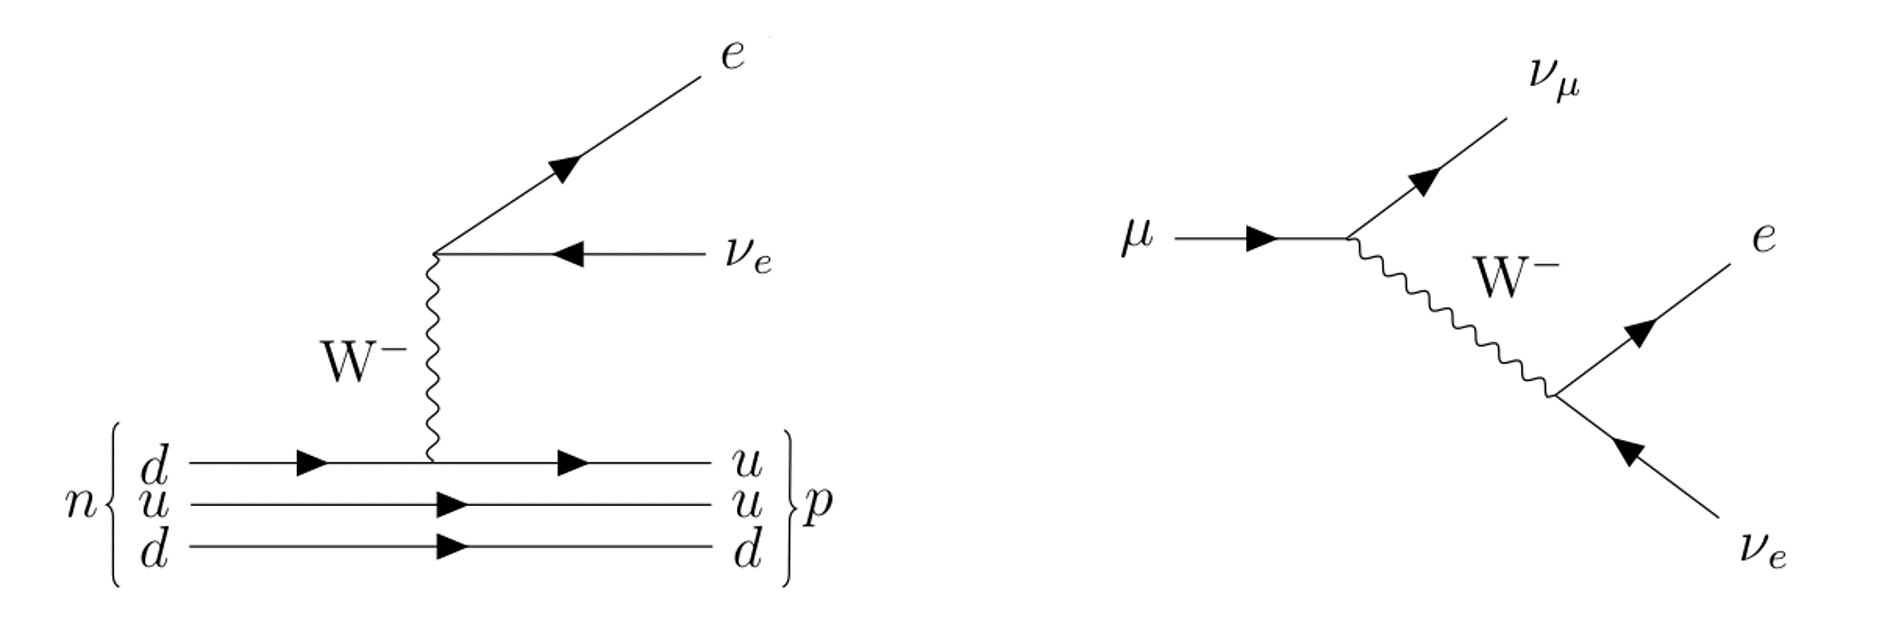
\includegraphics[width=0.9\textwidth]{figures/intro/neutron_muon_decays.pdf}
\caption{Long-lived decays of the neutron (left) and muon (right).}
\label{neutron_muon_decays}
\end{figure}

In BSM physics, the same fundamental mechanisms could very well produce new long-lived particles. Many SUSY scenarios, for example, introduce a symmetry known as R parity that prevents proton decay\fxnote{cite something, probably martin}. In models with exact R-parity conservation, SM particles are assigned R-parity \num{+1} and SUSY particles are assigned R-parity \num{-1}. Conserving the product of R-parity at each vertex has two phenomenological consequences: SUSY particles must be produced in pairs, and the lightest SUSY particle (LSP) must be absolutely stable. A neutral, weakly interacting LSP would therefore pass through most detectors (including the CMS detector described in Section~\ref{cms}) without interacting. The resulting momentum imbalance is a standard signature in many SUSY searches \cite{pdg_2020}.

On the other hand, SUSY models with weakly coupled R-parity violating (RPV) terms produce long-lived but not perfectly stable LSPs. The following section will give a detailed overview of one such model. A similar situation arises in gauge-mediated SUSY breaking models where the gravitino\fxnote{I never defined the graviton} is the LSP. The strength of the coupling between the next-to-LSP (NLSP) and the gravitino is inversely proportional to the energy scale at which SUSY is broken. A high SUSY breaking scale therefore suppresses the NLSP decay rate, making it long lived \cite{liu_2015}.

LLPs also arise from particular SUSY mass spectra. Models in the Split SUSY paradigm, for example, propose that the spin-0 SUSY particles are significantly more massive than the spin-$\frac{1}{2}$ SUSY particles. In these models, the gluino becomes long lived when its decay to two quarks and a neutral spin-$\frac{1}{2}$ SUSY particle is suppressed by a highly virtual intermediate squark \cite{split_susy_colliders}. Other SUSY models produce long-lived particles by limiting decay phase space. Some anomaly-mediated SUSY breaking models, for example, predict that the NLSP and LSP are nearly degenerate in mass. Just like the neutron decaying into a proton, the lack of available phase space suppresses the decay and produces a long-lived NLSP \cite{amsb_at_lhc}.

In summary, LLPs are a general feature of the SM, and it is reasonable to assume that the same mechanisms that produce SM LLPs will also manifest in BSM physics. The following subsection gives an overview of the phenomenology of the SUSY model most relevant to the analysis presented in Chapter~\ref{displaced_leptons}, while the experimental details of this model and LLP searches at the LHC will be saved until after presenting the LHC and CMS experiment in Chapter~\ref{lhc_and_cms}.

\subsection{Displaced supersymmetry}
As mentioned in Section~\ref{susy}, weak-scale SUSY has the potential to explain the seemingly unnatural observed value of the Higgs boson mass\fxnote{weak scale probably hasn't been defined yet}. With this appealing outcome in mind, experimental physicists have been searching for signs of SUSY in high-energy particle collisions for the last few decades\fxnote{cite some recent review and maybe some old lep or tevatron review (pdg susy chapter ain't bad)}. In particular, searches at the Large Hadron Collider, where the \num{7}, \num{8}, and \SI{13}{\TeV} proton-proton collisions could potentially be producing SUSY particles with masses above \SI{1}{\TeV}\fxnote{cite susy production xs? pdg figure 90.1 is nice}, are actively excluding large swaths of the natural SUSY parameter space. By examining the common assumptions behind a majority of these searches, the proponents of the Displaced SUSY model find an approach that avoids proton decay constraints while naturally producing long-lived SUSY particles that would be undetected by most collider searches \cite{displaced_susy}.

Displaced SUSY is an RPV SUSY model that respects proton lifetime constraints by allowing terms that violate lepton number but not baryon number. The Minimal Supersymmetric Standard Model, which is a simple supersymmetric extension of the SM, allows the following baryon and lepton violating operators:
\begin{equation}
    \label{lepton_baryon_violating_terms}
    \frac{1}{2}\lambda''_{ijk}U_{i}D_{j}D_{k},\ \frac{1}{2}\lambda_{ijk}L_{i}L_{j}E_{k},\  \lambda'_{ijk}L_{i}Q_{j}D_{k},\  \epsilon_{i}L_{i}H_{u} 
\end{equation}
where the first term violates baryon number and the remaining terms violate lepton number. The i, j, and k indices run over the three generations of fermions and $U$, $D$, $L$, $E$, $Q$, and $H$ refer to the SUSY multiplets whose SM components are right-handed up-type quarks, right-handed down-type quarks, left-handed leptons, right-handed leptons, left-handed quarks, and Higgs bosons, respectively \cite{susy_primer}. Most SUSY models introduce R-parity to forbid all of these terms and therefore disallow proton decay, but this approach may be overkill: separately conserving either lepton number or baryon number is sufficient to prevent\fxnote{prevent or slow?} proton decay.

Such a situation can arise naturally if a gauge-unifying, R-parity-conserving $SU(5)$ theory exists at high energies but is broken at lower energies \cite{hall_suzuki_rpv}. In this scenario, the baryon-number-violating terms are suppressed and mixing between $L$ and $H$ becomes possible. The final term in expression~\eqref{lepton_baryon_violating_terms} then dominates, and we are left with the following lepton-number-violating terms after rotating to the mass basis\fxnote{learn this better}:
\begin{equation}
    \label{displaced_susy_terms}
    \epsilon_{i}y^{d}_{jk}L_{i}Q_{j}D_{k},\ \epsilon_{i}y^{e}_{jk}L_{i}L_{j}E_{k} 
\end{equation}
where the $\epsilon$ factors are lepton-Higgs mixing angles and the $y$ factors are the SM Yukawa\fxnote{have I explained yukawa terms yet?} coupling constants. The presence of the Yukawa coupling constants implies that lepton-violating processes will favor third-generation fermions.
\fxnote{mention tree-level neutrino masses somewhere?}

The dimensionless lepton-Higgs mixing angles are protected by the custodial R-parity conservation of the higher-energy theory\fxnote{is this technically true? if not, can just say they're inversely proportional to $\Lambda$} and can therefore naturally be small. Just as in the SM, these small coupling constants can lead to macroscopic SUSY particle lifetimes that would evade most collider searches. In particular, long-lived LSP squarks can decay to a quark and charged lepton though a displaced vertex, as in Fig.~\ref{stop_to_lb}.

\begin{figure}
\centering
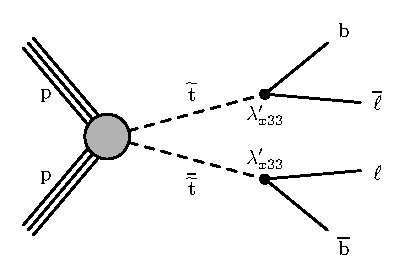
\includegraphics[width=0.5\textwidth]{figures/intro/stopToLB.pdf}
\caption{Pair-produced top squarks that each decay to a bottom quark and a lepton through an R-parity-violating $LQD$ vertex.}
\label{stop_to_lb}
\end{figure}

The unique experimental signature of processes such as the one shown in Fig.~\ref{stop_to_lb} is a major motivating factor behind the analysis presented in Chapter~\ref{displaced_leptons}. The particular experimental consequences of such processes will be further explored in that context.

\pagebreak